\documentclass[acmsmall,screen]{acmart}

%%% The following is specific to ICFP '19 and the paper
%%% 'Selective Applicative Functors'
%%% by Andrey Mokhov, Georgy Lukyanov, Simon Marlow, and Jeremie Dimino.
%%%
\setcopyright{rightsretained}
\acmPrice{}
\acmDOI{10.1145/3341694}
\acmYear{2019}
\copyrightyear{2019}
\acmJournal{PACMPL}
\acmVolume{3}
\acmNumber{ICFP}
\acmArticle{90}
\acmMonth{8}

\bibliographystyle{ACM-Reference-Format}
\citestyle{acmauthoryear}

%% Some recommended packages.
\usepackage{booktabs}   %% For formal tables:
                        %% http://ctan.org/pkg/booktabs
\usepackage{subcaption} %% For complex figures with subfigures/subcaptions
                        %% http://ctan.org/pkg/subcaption

\usepackage{bookmark}
\usepackage[utf8]{inputenc}
\usepackage[T1]{fontenc}
\usepackage{xspace}
\usepackage{fancyhdr}

% Haskell code snippets and useful shortcuts
\usepackage{minted}
\setminted[haskell]{escapeinside=@@}
\newcommand{\hs}{\mintinline{haskell}}
\newcommand{\cmd}[1]{\textsf{\color[rgb]{0,0,0.5} #1}}
\newcommand{\teq}{\smaller $\sim$}
\newcommand{\ghci}{$\lambda$>}
\newcommand{\defeq}{\stackrel{\text{def}}{=}}
\newcommand{\dollar}{{\color[rgb]{0.40,0.40,0.40} \$}}
\newcommand{\std}[1]{{\color[rgb]{0,0.3,0} #1}}
\newcommand{\blk}[1]{{\color[rgb]{0,0,0} #1}}
\newcommand{\blu}[1]{{\color[rgb]{0,0,1.0} #1}}

% Questions and tasks
\newcommand{\q}[2]{\textbf{\color{blue} Question #1:} #2}
\newcommand{\todo}[2]{[\textbf{\color{red} #1:} #2]}

% Abbreviations for projects
\newcommand{\Dune}{\textsc{Dune}\xspace}
\newcommand{\Haxl}{\textsc{Haxl}\xspace}

\begin{document}

%% Title information
\title{Selective Applicative Functors}

%% Sadly, it looks like we can't have a subtitle that doesn't also appear in the
%% ACM Reference.
% \subtitle{Declare Your Effects Statically, Select Which to Execute Dynamically}

\author{Andrey Mokhov}
\affiliation{
  \institution{Newcastle University}
  \country{United Kingdom}
}
\email{andrey.mokhov@ncl.ac.uk}
\author{Georgy Lukyanov}
\affiliation{
  \institution{Newcastle University}
  \country{United Kingdom}
}
\email{g.lukyanov2@ncl.ac.uk}
\author{Simon Marlow}
\affiliation{
  \institution{Facebook}
  \city{London}
  \country{United Kingdom}
}
\email{smarlow@fb.com}
\author{Jeremie Dimino}
\affiliation{
  \institution{Jane Street}
  \city{London}
  \country{United Kingdom}
}
\email{jdimino@janestreet.com}

% Don't forget \thispagestyle{firstpagestyle} after \maketitle
% \fancypagestyle{firstpagestyle}
% {
%    \fancyhf{}
%    \renewcommand{\headrulewidth}{0.2pt}
%    \fancyhead[C]{Under review, feedback is sought}
% }

\begin{abstract}
Applicative functors and monads have conquered the world of functional
programming by providing general and powerful ways of describing effectful
computations using pure functions. Applicative functors provide a way to compose
\emph{independent effects} that cannot depend on values produced by earlier
computations, and all of which are declared statically. Monads extend the
applicative interface by making it possible to compose \emph{dependent effects},
where the value computed by one effect determines all subsequent effects,
dynamically.

This paper introduces an intermediate abstraction called \emph{selective
applicative functors} that requires all effects to be declared statically, but
provides a way to select which of the effects to execute dynamically. We
demonstrate applications of the new abstraction on several examples, including
two industrial case studies.
\end{abstract}

%% 2012 ACM Computing Classification System (CSS) concepts
%% Generate at 'http://dl.acm.org/ccs/ccs.cfm'.
\begin{CCSXML}
<ccs2012>
<concept>
<concept_id>10011007</concept_id>
 <concept_desc>Software and its engineering</concept_desc>
<concept_significance>500</concept_significance>
</concept>
<concept>
<concept_id>10002950</concept_id>
 <concept_desc>Mathematics of computing</concept_desc>
<concept_significance>300</concept_significance>
</concept>
</ccs2012>
\end{CCSXML}
\ccsdesc[500]{Software and its engineering}
\ccsdesc[300]{Mathematics of computing}

\keywords{applicative functors, selective functors, monads, effects}

\maketitle
% \thispagestyle{firstpagestyle}

\section{Introduction}\label{sec-intro}

% , further referred to simply as \emph{effects}

Monads, introduced to functional programming by~\citet{1995_wadler_monads}, are
a powerful and general approach for describing effectful (or impure)
computations using pure functions. The key ingredient of the monad abstraction
is the \emph{bind} operator, denoted by \hs{>>=} in
Haskell\footnote{We use Haskell throughout this paper, but the presented results
are not specific to Haskell and do not require any advanced features of the
Glasgow Haskell Compiler (any Haskell98~\citep{haskell98} compliant compiler
will do). Furthermore, we release two libraries for selective applicative
functors along with this paper: for Haskell and OCaml.}:

\vspace{1mm}
\begin{minted}[xleftmargin=10pt]{haskell}
(>>=) :: Monad f => f a -> (a -> f b) -> f b
\end{minted}
\vspace{1mm}

\noindent
The operator takes two arguments: an effectful computation \hs{f}~\hs{a}, which
yields a value of type~\hs{a} when executed, and a recipe, i.e. a pure function
of type \hs{a}~\hs{->}~\hs{f}~\hs{b}, for turning~\hs{a} into a subsequent
computation of type \hs{f}~\hs{b}. This approach to composing effectful
computations is inherently sequential: until you execute the effects in
\hs{f}~\hs{a}, you have no way of obtaining the continuation \hs{f}~\hs{b},
i.e. these computations can only be performed in sequence.

Consider a simple example, where we use the monad \hs{f}~\hs{=}~\hs{IO} to
describe an effectful program that prints \hs{"pong"} if the user enters
\hs{"ping"}:

\vspace{1mm}
\begin{minted}[xleftmargin=10pt]{haskell}
pingPongM :: IO ()
pingPongM = getLine
            >>=
            \s -> if s == "ping" then putStrLn "pong" else pure ()
\end{minted}
\vspace{1mm}

\noindent
Here the first argument of the bind operator reads a string using
\hs{getLine}~\hs{::}~\hs{IO}~\hs{String}, and the second argument is the
function of type \hs{String}~\hs{->}~\hs{IO}~\hs{()}, which examines the string
and prints \hs{"pong"} if need be. While this works, the function is completely
opaque: there is no way to "see through" the lambda \hs{\s}~\hs{->}~\hs{...} to
predict the effects it might perform. Instead of conditionally executing
\hs{putStrLn}, as intended, it could delete a file from disk, or launch
proverbial missiles. As we will see in sections~\S\ref{sec-static}
and~\S\ref{sec-haxl}, in some applications it is desirable to know all possible
effects \emph{statically}, i.e. before starting the computation.

Applicative functors, introduced by~\citet{mcbride2008applicative}, can be used
for composing a statically known collection of effectful computations, as long
as these computations are \emph{independent}. The key ingredient of applicative
functors is the \emph{apply} operator, denoted by \hs{<*>}:

\vspace{1mm}
\begin{minted}[xleftmargin=10pt]{haskell}
(<*>) :: Applicative f => f (a -> b) -> f a -> f b
\end{minted}
\vspace{1mm}

\noindent
The operator takes two effectful computations, which -- independently -- compute
values of types \hs{a}~\hs{->}~\hs{b} and \hs{a}, and returns their composition
that performs both computations, and applies the obtained function to the
obtained value producing the result of type \hs{b}. Crucially, both arguments
and associated effects are known statically, which, for example, allows us to
allocate all necessary resources upfront (\S\ref{sec-static}) or execute both
computations in parallel (\S\ref{sec-haxl}).

Alas, our ping-pong example cannot be expressed using applicative functors.
Since the two computations must be independent, the best we can do is to print
\hs{"pong"} unconditionally:

\vspace{1mm}
\begin{minted}[xleftmargin=10pt]{haskell}
pingPongA :: IO ()
pingPongA = fmap (const id) getLine
            <*>
            putStrLn "pong"
\end{minted}
\vspace{1mm}

\noindent
We use \hs{fmap}~\hs{(}\hs{const}~\hs{id)} to replace the input string, which we
now have no need for, with the identity function to match the return type of
\hs{putStrLn}~\hs{::}~\hs{IO}~\hs{()}.


\section{Selective functors}\label{sec-selective}

\begin{figure}
\begin{minted}[fontsize=\small]{haskell}
class Functor f where
    fmap :: (a -> b) -> f a -> f b

-- An infix synonym for fmap
(<$>) :: Functor f => (a -> b) -> f a -> f b       -- (<$>) is pronounced as "map"

class Functor f => Applicative f where
    pure  :: a -> f a
    (<*>) :: f (a -> b) -> f a -> f b              -- (<*>) is pronounced as "apply"

-- A variant of <*> with the arguments reversed
(<**>) :: Applicative f => f a -> f (a -> b) -> f b

class Applicative f => Selective f where
    select :: f (Either a b) -> f (a -> b) -> f b

-- An infix synonym for select
(<*?) :: f (Either a b) -> f (a -> b) -> f b       -- (<*?) is pronounced as "select"

class Selective f => Monad f where
    return :: a -> f a
    (>>=)  :: f a -> (a -> f b) -> f b             -- (>>=) is pronounced as "bind"
\end{minted}
\caption{The proposed type class hierarchy, where \hs{Functor}, \hs{Applicative}
and \hs{Monad} are standard Haskell type classes, and \hs{Selective} is
a new intermediate abstraction introduced between \hs{Applicative} and
\hs{Monad}.}\label{fig-types}
\end{figure}

In this section we introduce selective applicative functors, which we will
further refer to as simply \emph{selective functors}, for brevity. We start by
defining the new abstraction and using it to implement several simple
combinators, such as the aforementioned \hs{whenS}. In~\S\ref{sec-instances} we
provide several examples of selective functors, and discuss the relationships
between applicative functors, selective functors, and monads.
In~\S\ref{sec-laws}, these relationships are further elaborated and expressed
as a set of laws that all selective functors are required to satisfy.

Like applicative functors~\citep{mcbride2008applicative}, selective functors
provide a way to embed pure values into an effectful context \hs{f} using the
function \hs{pure}, and give meaning to composition of two independent effectful
computations using the operator \hs{<*>}. See Fig.~\ref{fig-types} for the
standard definition of the corresponding type class \hs{Applicative}. Selective
functors enrich the applicative interface with the \hs{select} function, which
gives meaning to the composition of two effectful computations, where, in
contrast to \hs{<*>}, the second computation \emph{may depend} on the first one:

\vspace{1mm}
\begin{minted}[xleftmargin=10pt]{haskell}
class Applicative f => Selective f where
    select :: f (Either a b) -> f (a -> b) -> f b
\end{minted}
\vspace{1mm}

\noindent
One can think of \hs{select} as a selective function application:
parametricity~\citep{wadler1989theorems} dictates that we \emph{must apply} the
function of type \hs{a}~\hs{->}~\hs{b} when given a value of type
\hs{Left}~\hs{a}, but we \emph{may skip} the function and associated effects,
and simply return the \hs{b} when given a \hs{Right}~\hs{b}. Following the
notational convention for applicative operators, we also define the infix
operator alias \hs{<*?} for \hs{select}: the angle bracket pointing to the left
means we always use the corresponding value; the value on the right, however,
may be skipped, hence the question mark.

Note that one can implement a function with the type signature of \hs{select}
using applicative functors, but it will always execute the effects associated
with the second argument, rendering any conditional execution of effects
impossible, as in the \hs{pingPongA} example in~\S\ref{sec-intro}:

\vspace{1mm}
\begin{minted}[xleftmargin=10pt]{haskell}
selectA :: Applicative f => f (Either a b) -> f (a -> b) -> f b
selectA x y = (\e f -> case e of { Left a -> f a; Right b -> b }) <$> x <*> y
\end{minted}
\vspace{1mm}

\noindent
As we will see in~\S\ref{sec-instances}, the above definition is sometimes
useful, for example, selective functors used for static analysis need to collect
information about all possible effects instead of skipping some of them,
therefore directly using \hs{select}~\hs{=}~\hs{selectA} in their
\hs{Selective} instance definition.

As a first use-case of selective functors, let us revisit our ping-pong example
from~\S\ref{sec-intro} and implement the combinator \hs{whenS}:

\vspace{1mm}
\begin{minted}[xleftmargin=10pt]{haskell}
whenS :: Selective f => f Bool -> f () -> f ()
whenS x y = selector <*? effect
  where
    selector = fmap (\b -> if b then Left () else Right ()) x
    effect   = fmap const                                   y
\end{minted}
\vspace{1mm}

\noindent
We first bring the given effectful computations into the right shape by using
the \hs{Functor}'s function \hs{fmap} (see
Fig.~\ref{fig-types}); specifically, \hs{x}~\hs{::}~\hs{f}~\hs{Bool} is
converted into a \hs{selector}~\hs{::}~\hs{f}~\hs{(Either}~\hs{()}~\hs{())}, and
\hs{y}~\hs{::}~\hs{f}~\hs{()} is converted into
\hs{effect}~\hs{::}~\hs{f}~\hs{(()}~\hs{->}~\hs{())}. The results are composed
using the select operator \hs{<*?}, and the meaning of this composition is
determined by a specific \hs{Selective} instance.
% (see some examples in~\S\ref{sec-instances}).

It is worth noting that unlike the select operator, whose implementation is
almost completely determined by parametricity (the only real question is:
\emph{"To skip, or not to skip?"}), \hs{whenS} admits a variety of (incorrect)
implementations. In particular, due to \emph{Boolean blindness}\footnote{The
term refers to the fact that the \hs{True} and \hs{False} values are not
distinguished at the type level, see~\citet{boolean-blindness}.},
it is easy to inadvertently implement \hs{unlessS}, which has the same type but
flips the meaning of the Boolean value. The ability to reason parametrically was
one of the guiding principles we used when looking for a good abstraction for
selective functors: \hs{select} provides this ability, whereas \hs{whenS} does
not.
% Constraints liberate, liberties constrain

A strong contender for being the main ingredient of selective functors is the
function \hs{branch} that, given an effectful computation
\hs{x}~\hs{::}~\hs{f}~\hs{(Either}~\hs{a}~\hs{b)}, selects which subsequent
computation, namely \hs{l}~\hs{::}~\hs{f}~\hs{(}\hs{a}~\hs{->}~\hs{c)} or
\hs{r}~\hs{::}~\hs{f}~\hs{(}\hs{b}~\hs{->}~\hs{c)}, to execute:

\vspace{1mm}
\begin{minted}[xleftmargin=10pt]{haskell}
branch :: Selective f => f (Either a b) -> f (a -> c) -> f (b -> c) -> f c
branch x l r = fmap (fmap Left) x <*? fmap (fmap Right) l <*? r
\end{minted}
\vspace{1mm}

\noindent
While we encourage the reader to derive this implementation as an exercise, we
would like to also share our intuition behind it, as it will be useful for
\emph{free selective functors} in~\S\ref{sec-free}.
The select operator allows us to eliminate one of the cases in a sum type,
namely the \hs{Left}~\hs{a} case in \hs{Either}~\hs{a}~\hs{b}, leaving the other
case intact. To implement \hs{branch}, we will need to apply \hs{<*?} twice,
eliminating \hs{a} and \hs{b} one after another. The first application is tricky
because \hs{f}~\hs{(Either}~\hs{a}~\hs{b)} and
\hs{f}~\hs{(}\hs{a}~\hs{->}~\hs{c)} do not match the type signature of \hs{<*?}.
To fix the mismatch, we convert them to
\hs{f}~\hs{(Either}~\hs{a}~\hs{(}\hs{Either}~\hs{b}~\hs{c))} and
\hs{f}~\hs{(}\hs{a}~\hs{->}~\hs{Either}~\hs{b}~\hs{c)}, respectively. The second
application of \hs{<*?} is then straightforward.

As discussed in~\S\ref{sec-alternatives}, we could have chosen to use
\hs{branch} instead of \hs{select} as the method of the \hs{Selective} type
class. Our choice of \hs{select} followed the Occam's razor principle:
\hs{select} is simpler than \hs{branch}, which, in particular, leads to a
simpler free construction (\S\ref{sec-free}).

By instantiating \hs{select} to \hs{a}~\hs{=}~\hs{b}~\hs{=}~\hs{()} we obtained
\hs{whenS}, and now we repeat this trick, obtaining another familiar combinator
\hs{ifS} from the function \hs{branch}:

\vspace{1mm}
\begin{minted}[xleftmargin=10pt]{haskell}
ifS :: Selective f => f Bool -> f a -> f a -> f a
ifS i t e = branch (bool (Right ()) (Left ()) <$> i) (const <$> t) (const <$> e)
\end{minted}
\vspace{1mm}

\subsection{Basic examples}\label{sec-instances}

Over, under

Validation

\subsection{Laws}\label{sec-laws}

It may be illuminating to compare the following type signatures:

\begin{minted}[xleftmargin=10pt]{haskell}
(<**>) :: Applicative f => f a            -> f (a -> b) -> f b
select :: Selective   f => f (Either a b) -> f (a -> b) -> f b
(>>=)  :: Monad       f => f a            -> (a -> f b) -> f b
\end{minted}

The type signature of \hs{select} is reminiscent of both \hs{<*>} and \hs{>>=},
and indeed a selective functor is in some sense a composition of an applicative
functor and the \hs{Either} monad.


Note that it is not a requirement for selective functors to skip unnecessary
effects. It may be counterintuitive, but this makes them more useful. Why?
Typically, when executing a selective computation, you would want to skip the
effects (saving work); but on the other hand, if your goal is to statically
analyse a given selective computation and extract the set of all possible
effects (without actually executing them), then you do not want to skip any
effects, because that defeats the purpose of static analysis.

...

\begin{figure}
\begin{minted}[fontsize=\small]{haskell}
branch :: Selective f => f (Either a b) -> f (a -> c) -> f (b -> c) -> f c
branch x l r = fmap (fmap Left) x <*? fmap (fmap Right) l <*? r

ifS :: Selective f => f Bool -> f a -> f a -> f a
ifS i t e = branch (bool (Right ()) (Left ()) <$> i) (const <$> t) (const <$> e)

whenS :: Selective f => f Bool -> f () -> f ()
whenS x act = ifS x act (pure ())

whileS :: Selective f => f Bool -> f ()
whileS act = whenS act (whileS act)

(<||>) :: Selective f => f Bool -> f Bool -> f Bool
(<||>) a b = ifS a (pure True) b

(<&&>) :: Selective f => f Bool -> f Bool -> f Bool
(<&&>) a b = ifS a b (pure False)

anyS :: Selective f => (a -> f Bool) -> [a] -> f Bool
anyS p = foldr ((<||>) . p) (pure False)

allS :: Selective f => (a -> f Bool) -> [a] -> f Bool
allS p = foldr ((<&&>) . p) (pure True)
\end{minted}
\caption{Various conditional combinators implemented using selective functors.}
\label{fig-library}
\end{figure}
\section{Static analysis}\label{sec-static}

In this section we discuss a real-life application that benefits from static
analysis of effectful computations -- the \Dune build system~\citep{dune}. We
start by introducing \Dune and motivating the need for static analysis with
over-approximation (\S\ref{sec-dune-intro}), and then show how one can implement
static analysis of build system dependencies using selective functors
(\S\ref{sec-static-example}).

\subsection{Dune build system}\label{sec-dune-intro}

\Dune was originally developed at Jane Street and has by now become a standard
build system for OCaml packages~\citep{dune}. At the time of writing, more than
1000 OCaml packages are using Dune as the build system. The original motivation
for developing \Dune (earlier known as \textsf{jbuilder}) was to make it easier
to open source code developed in an industrial environment, and so \Dune was not
meant to be used for everyday software development. However, \Dune's ability to
extract maximum parallelism from build scripts meant it was faster than existing
build systems, such as OCamlbuild, and it quickly became popular, with major
projects switching to \Dune, for example, the Coq proof
assistant~\citep{bertot2013coq}.

% TODO: Can we get any performance improvement figures on how much more
% parallelism can be gained through static analysis?

One unusual feature of \Dune is the ability to statically over-approximate all
build dependencies of a package instead of requiring the programmer to manually
list them in a \emph{package manifest file}. Package manifest files are consumed
by \emph{package managers}, such as OPAM~\citep{opam} for the purpose of
downloading and installing all required dependencies.

% The original aim of this feature was to automatically generate package manifest
% files, so that they do not need to be maintained. An alternative approach would
% be to integrate the build system with the package manager itself, i.e. whenever
% the build system discovers a new external dependency, the package manager would
% download and install it, temporarily suspending the build.

% The reason Dune could not follow this approach is because package managers are
% typically designed to be build system agnostic.

% There are also optional package dependencies. Shall we give more details?

To generate a manifest file automatically \Dune needs to analyse the build graph
statically, i.e. \emph{without actually running any build commands}, because at
this point the project cannot yet be built (due to missing dependencies).
Package dependencies can be conditional and depend on values that can only be
computed during the build, therefore in many situations it is impossible to
statically compute an exact set of dependencies, and hence an over-approximation
is used instead.

In general, one can view such static dependency analysis as a function from a
build script to a set of package dependencies, and implement it directly by
parsing the script and extracting all possible dependencies from it. \Dune
adopts a different approach: it reuses the existing script execution engine that
executes build commands, but in a mock environment where commands are skipped,
but their dependencies are recorded in all branches of conditional statements.
By doing static analysis at this level, one can reuse a lot of code, e.g. for
parsing and interpreting build scripts.

% giving us good confidence in these parts of the implementation.

In this mock environment, some parts of the code cannot be fully evaluated as
they need the output produced by external commands. However, these parts still
need to be analysed. To achieve this, the original implementation of \Dune uses
the \emph{arrow} abstraction discussed in~\S\ref{sec-arrows}. To evaluate
suitability of selective functors for this task, we have successfully prototyped
an alternative core for \Dune, which uses applicative and selective functors
instead of arrows.

% The reason Dune uses an arrow
% rather than an applicative is discussed later, however applicatives
% would be suitable as well in this context. In particular, a
% successful attempt was made at replacing arrows by applicatives in
% Dune in the past.

\subsection{Static analysis of build dependencies}\label{sec-static-example}

\Dune is written in OCaml, and we therefore developed an OCaml library for
selective functors. In this section, however, we choose to continue using
Haskell to avoid confusion.

We follow the approach by~\citet{mokhov2018build} for modelling \emph{build
tasks}, where a single task is represented as a higher-order effectful function
parameterised by the type of \emph{keys} \hs{k}, e.g. file names, and the type
of \emph{values} \hs{v}, e.g. file contents. A task takes a \emph{callback} of
type \hs{k}~\hs{->}~\hs{f}~\hs{v}, that the task can use to find values of its
dependencies, and returns the result embedded in a selective context~\hs{f}:

\vspace{1mm}
\begin{minted}[xleftmargin=10pt]{haskell}
newtype Task k v = Task { run :: forall f. Selective f => (k -> f v) -> f v }
\end{minted}
\vspace{1mm}

\noindent
The task needs to be polymorphic over the \hs{f} so that it can be run both in
\emph{build mode}, by actually executing build commands, and in the \emph{mock
mode}, where build commands are skipped but dependencies are recorded, as
explained in \S\ref{sec-dune-intro}. For example, to compute over- and
under-approximation of build dependencies we can run the task in selective
functors \hs{f}~\hs{=}~\hs{Over} and \hs{f}~\hs{=}~\hs{Under}, respectively:

\vspace{1mm}
\begin{minted}[xleftmargin=10pt]{haskell}
dependenciesOver :: Task k v -> [k]
dependenciesOver task = getOver $ run task (\k -> Over [k])

dependenciesUnder :: Task k v -> [k]
dependenciesUnder task = getUnder $ run task (\k -> Under [k])
\end{minted}
\vspace{1mm}

\noindent
Thanks to the polymorphism of the task description over \hs{f}, we can
``execute'' a given task with a mock callback like
\hs{(\}\hs{k}~\hs{->}~\hs{Over}~\hs{[}\hs{k])}~\hs{::}~\hs{k}~\hs{->}~\hs{Over}~\hs{v},
whose only effect is recording the given key.

To demonstrate this on an example, we need a way to model a \emph{build script},
i.e. a collection of build tasks. One simple approach~\citep{mokhov2018build}
is to use a function that, given a key~\hs{k} returns either the corresponding
build \hs{Task} or \hs{Nothing} to indicate that this key is an input~(external)
dependency that cannot be built and should therefore be available before the
build starts:

\vspace{1mm}
\begin{minted}[xleftmargin=10pt]{haskell}
type Script k v = k -> Maybe (Task k v)
\end{minted}
\vspace{1mm}

\noindent
Now we have all the ingredients for creating a simple build script comprising
two tasks: (i)~the top-level task for building \cmd{release.tar} by archiving
the file \cmd{LICENSE} and the executable \cmd{exe}; and (ii)~the task for
compiling the executable from the source \cmd{src.ml} and one of the two
libraries: \cmd{lib.c} or \cmd{lib.ml}, depending on the configuration option
stored in the \cmd{config} file (it is common to use an optimised low-level C
implementation of a performance-critical function, falling back to high-level
OCaml implementation if the former is unavailable on the system):

\vspace{1mm}
\begin{minted}[xleftmargin=10pt]{haskell}
script :: Script FilePath String
script "release.tar" = Just $ Task $ \fetch -> tar [fetch "LICENSE", fetch "exe"]
script "exe" = Just $ Task $ \fetch ->
    let src  = fetch "src.ml"
        cfg  = fetch "config"
        lib1 = fetch "lib.c"
        lib2 = fetch "lib.ml"
    in compile [src, ifS (parse cfg) lib1 lib2]
script _ = Nothing
\end{minted}
\vspace{1mm}

\noindent
We assume the existence of functions \hs{tar} (creating an archive),
\hs{compile} (compiling an OCaml executable from source and libraries), and
\hs{parse} (parsing a configuration file); their implementation is irrelevant
for our purposes.

\begin{figure}
\centerline{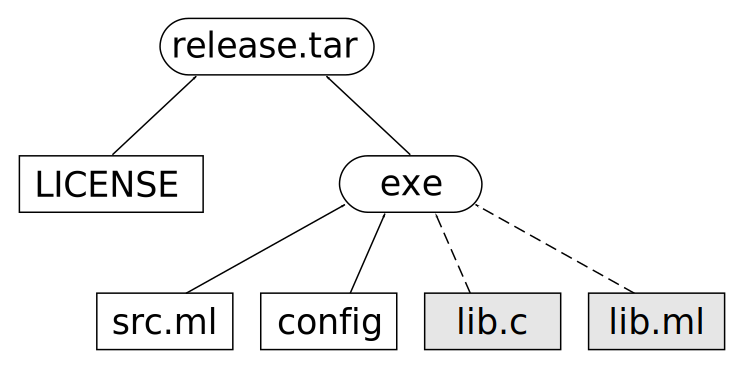
\includegraphics[scale=0.3]{fig/build-dependencies.pdf}}
\caption{An example build dependency graph. Input files are shown in rectangles,
intermediate and output files are shown in rounded rectangles. Approximate
dependencies are highlighted with dashed lines.}
\label{fig-build}
\end{figure}

By analysing individual build tasks using \hs{dependenciesOver} and
\hs{dependenciesUnder}, we can obtain an approximate build dependency
information for the whole dependency graph:

\vspace{1mm}
\begin{minted}[xleftmargin=10pt]{haskell}
@\ghci@ dependenciesOver (fromJust $ script "release.tar")
["LICENSE","exe"]
@\ghci@ dependenciesUnder (fromJust $ script "release.tar")
["LICENSE","exe"]
@\ghci@ dependenciesOver (fromJust $ script "exe")
["src.ml","config","lib.c","lib.ml"]
@\ghci@ dependenciesUnder (fromJust $ script "exe")
["src.ml","config"]
\end{minted}
\vspace{1mm}

\noindent
Fig.~\ref{fig-build} visualises the graph obtained by traversing approximate
dependencies starting from the target key \cmd{release.tar}.

Note that while over-approximation is useful for installing all possible
dependencies \emph{before the build}, under-approximation is useful for
maximising parallelism \emph{during the build}: for example, if all input files
in our example are actually generated, e.g. by running a text preprocessor, then
we can start the three preprocessing tasks that are definitely needed
(\cmd{LICENSE}, \cmd{src.ml}, \cmd{config}) in parallel, i.e. without waiting
for the outcome of parsing the \cmd{config} file.

\emph{Applicative and monadic build systems} studied in~\citep{mokhov2018build}
cannot support such over- and under-approximating static analysis, and the
associated abstractions are therefore unsuitable for \Dune. This explains why
\Dune developers have chosen to use the \emph{arrow} abstraction
(\S\ref{sec-arrows}). As our case study and the developed prototype demonstrate,
selective functors provide a viable alternative to arrows in the context of
build systems.

% Dune is another example where the extra power provided by selective
% functions is relevant. To understand why, let's consider the following
% example: a user wants to use some optimized C function if it is
% available on the system, and fallback to an OCaml implementation if
% not. The C and OCaml implementations might have different external
% dependencies. Such a test is dynamic since it depends on the system
% the users builds the software on. During compilation, we only want to
% follow one of the branch, as we clearly don't want to build
% implementation only to keep a single one. However, during dependency
% analysis for the project manifest we need to scan both branches. The
% dependencies discovered in both branches will be considered as
% optional dependencies given that neither is always required.

% For parallelism use underapproximation: take intersection of optional
% dependencies, and then union with necessary dependencies.

\section{Speculative execution}\label{sec-haxl}

\Haxl~\citep{marlow2014haxl} is a framework for efficiently executing
code that fetches data from external sources, typically databases or
remote services. The \Haxl framework allows code written in a natural
style using \hs{Applicative} and \hs{Monad} combinators to run
efficiently, by automatically parallelising the data fetch operations
and batching together multiple fetches from the same data source.

\Haxl has been in use at Facebook, at scale, for several years now in
a system that proactively detects and remediates various forms of
abuse. \Haxl allows the engineers working on the anti-abuse code to
write clear and concise application logic, because the framework
abstracts away from the details of concurrency and efficient
data-fetching.

To illustrate the idea using a fragment of the example code from
\citep{marlow2014haxl}, suppose we're writing the code to render a blog into
HTML. The blog consists of a set of posts, where each post is
identified by a \hs{PostId}.  The data for the blog is stored in a
remote database.  The API for fetching the data from the database is
as follows:

\begin{minted}[fontsize=\small]{haskell}
getPostIds     :: Haxl [PostId]
getPostContent :: PostId -> Haxl PostContent
\end{minted}

We can fetch the set of all \hs{PostId}s using \hs{getPostIds}, and we
can fetch the content of one post using \hs{getPostContent}. To get
the content of all posts we could write:

\begin{minted}[fontsize=\small]{haskell}
getAllPostsContent :: Haxl [PostContent]
getAllPostsContent = mapM getPostContent =<< getPostIds
\end{minted}

Now, when we \hs{mapM getPostContent} we would really like the
database queries to happen in parallel, because there are no
dependencies between them. Furthermore, we might even be able to batch
up the queries into a single request to the remote database.

These optimisations are performed automatically by \Haxl, using a
special instance of \hs{Applicative} that exploits the lack of
dependency between the two computations to explore the computations
and collect the data fetch operations that can be performed in
parallel or batched together. \Haxl also has a \hs{Monad} instance
that sequentializes operations as you would expect, but code written
to use \hs{Applicative} operations benefits from the automatic
concurrency. This optimisation is further exploited by using a
transformation on the monadic \hs{do} syntax to automatically use
\hs{Applicative} operators where possible \cite{applicative-do}.

One of the key tools found to be useful in the kind of code written
using \Haxl at Facebook is the ``lazy'' conditional operators:

\begin{minted}[fontsize=\small]{haskell}
(.||) :: Haxl Bool -> Haxl Bool -> Haxl Bool
x .|| y = do b <- x; if b then return True else y

(.&&) :: Haxl Bool -> Haxl Bool -> Haxl Bool
x .&& y = do b <- x; if b then y else return False
\end{minted}

These are typically used to improve performance by guarding expensive
checks with cheaper checks.  For example, we might write:

\begin{minted}[fontsize=\small]{haskell}
myDetector =
  if cheapCondition .&& expensiveCondition
    then ...
    else ...
\end{minted}

\noindent The idea is that \hs{cheapCondition} is cheap to evaluate and
returns \hs{False} in a large proportion of cases, so that we can
often avoid needing to evaluate \hs{expensiveCondition}.

This doesn't require any additional extensions or special support in
Haxl. But we also noticed that sometimes there is a pair of conditions
where neither is obviously cheaper than the other, yet we would still
like to benefit from bailing out early when the answer is known.
Therefore, \Haxl contains two more conditional operators \hs{pOr} and
\hs{pAnd} for ``parallel Or'' and ``parallel And'' respectively:

\begin{minted}[fontsize=\small]{haskell}
pOr, pAnd :: Haxl Bool -> Haxl Bool -> Haxl Bool
\end{minted}

These have the behaviour that

\begin{itemize}
\item Both arguments are evaluated in parallel.
\item The computation is aborted as soon as the answer is known, even
  if the other argument has not completed evaluation yet.
\end{itemize}

Data-fetches are not observable effects, so the parallelism is not
observable to the programmer (this is the property that \Haxl relies
on for the soundness of its parallel \hs{Applicative}
instance). However, \hs{pOr} and \hs{pAnd} are non-deterministic with
respect to exceptions: if an exception is thrown by either side, it
will be thrown by the computation as a whole immediately without
waiting for the other side to complete.  One could imagine an
alternative implementation which waits for the completion of the other
argument when an exception is raised; this would be deterministic, but
would be less efficient in the case of exceptions.

It should come as no surprise that \hs{pOr} and \hs{pAnd} can be
implemented using \hs{select}, indeed \hs{pOr = (<||>)} and \hs{pAnd =
  (<&&>)}.  An implementation of \hs{select} in terms of the \Haxl
implementation from \citet{marlow2014haxl} is given in
Figure~\ref{fig-haxl-select}.  For the purposes of the presentation
here we have renamed \hs{Fetch} to \hs{Haxl} and added support for
exceptions in the form of the \hs{Throw} cases.

\begin{figure}
\begin{minted}[fontsize=\small]{haskell}
instance Selective Haxl where
  select (Haxl x) (Haxl f) = Haxl $ do
    rx <- x
    case rx of
      Done (Right b) -> return (Done b)
      Done (Left  a) -> unHaxl (($a) <$> Haxl f)
      Throw e -> return (Throw e)
      Blocked br1 c -> do
        rf <- f
        case rf of
          Done f  -> unHaxl (either f id <$> c)
          Throw e -> return (Blocked br1 (select c (Haxl (return rf))))
          Blocked br2 d -> return (Blocked (br1 <> br2) (select c d)
\end{minted}
\caption{An implementation of \hs{Selective} for \hs{Haxl}}
\label{fig-haxl-select}
\end{figure}

There is one wrinkle with implementing \hs{pOr} and \hs{pAnd}
in terms of \hs{select}. Ideally, \hs{pOr} and \hs{pAnd} would be
symmetric: just as we can abort the right argument if the left
argument determines the answer, we should be able to abort the left
argument in the same way. Yet \hs{select} is inherently left-biased:
it requires that all the effects of the first argument are performed.
In Section~\ref{sec-alt-either} we will consider an alternative
combinator related to \hs{select} that will allow this kind of
symmetry to be expressed.

In \Haxl we found \hs{pOr} and \hs{pAnd} to be occasionally useful by
themselves, but a more compelling use case is when there is a list of
conditionals, where we can use the \hs{anyS} and \hs{allS}
combinators.  When there are a large number of conditions it becomes
very hard to manually order them effectively using \hs{.||},
especially when the set of conditions changes often. In this case
\hs{anyS} is very useful as a way to extract performance in a
non-invasive way.


\section{Free Selective Functors}\label{sec-free}

The idea of describing effectful computations using \emph{free constructions},
such as \emph{free}~\cite{swierstra2008data} and \emph{freer
monads}~\cite{kiselyov2015freer} and \emph{free applicative
functors}~\cite{free-applicatives} is well-studied in the functional programming
community. Free constructions allow us to focus on the internal aspects of the
effect under consideration and receive the desired applicative or monadic
computation structure \emph{for free}, i.e. without the need to define custom
instances or prove laws.

In this section we apply this idea to selective functors. We present a free
construction for \emph{rigid} selective functors
(\S\ref{sec-free-construction}), and demonstrate it on two examples
in~\S\ref{sec-free-ping-pong} and~\S\ref{sec-free-isa}.

\subsection{Free Construction}\label{sec-free-construction}

In the free structures methodology, the essence of an effect is captured by a
data type that encodes the ``commands'' which the effect provides, acting as a
deep embedding of the effect's interface. This data type needs only have enough
structure to be a~\hs{Functor}. The purpose of a free construction is then to
build a richer structure on top of this \emph{base functor}, which would have
the desired instances, in our case \hs{Applicative} and \hs{Selective}. In this
section we will denote the base functor by \hs{f}.

\begin{figure}
\begin{minted}[fontsize=\small]{haskell}
data Select f a where
    Pure   :: a -> Select f a
    Select :: Select f (Either a b) -> f (a -> b) -> Select f b
\end{minted}
\vspace{0mm}
\begin{minted}[fontsize=\small]{haskell}
instance Functor f => Functor (Select f) where
    fmap f (Pure a)     = Pure (f a)
    fmap f (Select x y) = Select (fmap f <$> x) (fmap f <$> y) -- Free theorem from Fig. 4
\end{minted}
\vspace{0mm}
\begin{minted}[fontsize=\small]{haskell}
instance Functor f => Applicative (Select f) where
    pure  = Pure
    (<*>) = apS -- Law of rigid selective functors
\end{minted}
\vspace{0mm}
\begin{minted}[fontsize=\small]{haskell}
instance Functor f => Selective (Select f) where
    select x (Pure y)     = either y id <$> x -- Generalised identity
    select x (Select y z) = Select (select (f <$> x) (g <$> y)) (h <$> z) -- Associativity
      where
        f x = Right <$> x
        g y = \a -> bimap (,a) ($a) y
        h z = uncurry z
\end{minted}
\vspace{0mm}
\begin{minted}[fontsize=\small]{haskell}
-- Lift a base functor into Select
liftSelect :: Functor f => f a -> Select f a
liftSelect f = Select (Pure (Left ())) (const <$> f)
\end{minted}
\vspace{0mm}
\begin{minted}[fontsize=\small]{haskell}
-- Interpret a free selective structure given a natural transformation from f to g
runSelect :: Selective g => (forall x. f x -> g x) -> Select f a -> g a
runSelect _ (Pure a)     = pure a
runSelect t (Select x y) = select (runSelect t x) (t y)
\end{minted}
\vspace{0mm}
\begin{minted}[fontsize=\small]{haskell}
-- Extract the resulting value from a pure selective computation
getPure :: Select f a -> Maybe a
getPure = runSelect (const Nothing)
\end{minted}
\vspace{0mm}
\begin{minted}[fontsize=\small]{haskell}
-- Extract all possible effects from a selective computation
getEffects :: Functor f => Select f a -> [f ()]
getEffects = getOver . runSelect (Over . pure . void)
\end{minted}
\vspace{-3mm}
\caption{A basic implementation of free rigid selective functors; various
improvements are omitted for clarity.}\label{fig-free}
\vspace{-3mm}
\end{figure}

As we remarked in~\S\ref{sec-laws}, rigid selective functors have a particularly
simple normal form thanks to the additional law \hs{(<*>)}~\hs{=}~\hs{apS},
which tells us that the apply operator \hs{<*>} is redundant and can be
implemented via the selective interface. This normal form has the following
linear structure:

\vspace{1mm}
\begin{minted}[xleftmargin=10pt]{haskell}
pure x <*? fa <*? fb <*? ... <*? fy
  where
    x  :: Either a (Either b (Either c (... z)))
    fa :: f (a ->   Either b (Either c (... z)))
    fb :: f (b ->             Either c (... z))
    ...
    fy :: f (y ->                           z)
\end{minted}
\vspace{1mm}

\noindent
In words, any rigid selective computation can be rewritten as a left-associated
sequence of select operators, where the initial pure value~\hs{x} belongs to a
large sum type (comprising alternatives~\hs{a}~to~\hs{z} in the above snippet),
and each of the subsequent effects eliminates one of the alternatives, in order,
until only one remains (namely, \hs{z}).

Interestingly, there is no right-associated version of the normal form because
the associativity law~(\S\ref{sec-laws}) can only be used to re-associate an
expression to the left, which is a consequence of the asymmetry of the select
operator. It is worth noting that this is different from applicative functors
that have two normal forms corresponding to left and right
re-association of the apply operator~\citep{free-applicatives}. A symmetric
version of the select operator, which can be re-associated in either direction,
is discussed in~\S\ref{sec-alt-symmetric}.

% To apply it in reverse, we would need to ``factor out'' the reshaping functions
% \hs{f}, \hs{g} and \hs{h} from the base functor, which is not always possible.

% To see why, consider the expression
% \hs{pure}~\hs{(Right}~\hs{(Left}~\hs{1))}~\hs{<*?}~\hs{p}~\hs{<*?}~\hs{q}, where
% the effect \hs{p} is unnecessary due to the leading selector \hs{Right}. It is
% not possible to re-associate this expression into
% \hs{pure}~\hs{(Right}~\hs{(Left}~\hs{1))}~\hs{<*?}~\hs{(@@p'}~\hs{<*?}~\hs{q')}
% because in the sub-expression \hs{(@@p'}~\hs{<*?}~\hs{q')} the first effect
% \hs{p'} cannot be skipped.

Fig.~\ref{fig-free} gives an encoding of this normal form in Haskell. The free
data type \hs{Select} represents a selective computation as a type-aligned
sequence of base functor effects, with the \hs{Pure} constructor at the head.
Instance definitions rely on the selective laws from~\S\ref{sec-laws},
specifically: generalised identity, associativity, and one of the free theorems.
We do not use distributivity as it is subsumed by the law of rigid selective
functors \hs{(<*>)}~\hs{=}~\hs{apS}, used in the \hs{Applicative} instance.

Effects of the base functor can be embedded in the free construction using
the helper function \hs{liftSelect}. To interpret a free selective computation
\hs{Select}~\hs{f}~\hs{a} in a selective functor \hs{g}, one needs to provide
a \emph{natural transformation} from \hs{f} to \hs{g} to the function
\hs{runSelect}, which traverses the sequence of effects, converts them to
\hs{g}, and composes the results using \hs{g}'s select operator.

For example, \hs{getPure} reinterprets a given free computation in the selective
functor \hs{g}~\hs{=}~\hs{Maybe} using the natural transformation
\hs{const}~\hs{Nothing}, which leaves the \hs{Pure} head of the sequence as is,
but turns any subsequent effect into \hs{Nothing}. Similarly, \hs{getEffects}
records all effects by stashing them in the selective functor \hs{Over}, which
are subsequently extracted from it by \hs{getOver}.

We can improve the encoding in~Fig.~\ref{fig-free} in several ways: (i)~make it
``freer'' by not requiring~\hs{f}~to be a~\hs{Functor}; (ii)~make \hs{fmap} and
\hs{select} asymptotically faster using the ideas
by~\citet{menendez2013free}; and (iii)~drop the rigidity requirement,
obtaining a general free construction for selective functors~---~see an
implementation in the library~\citep{selective2019haskell} and the supplementary
material.

\subsection{Ping-pong, Freely}\label{sec-free-ping-pong}

To illustrate the usage of free selective functors on a simple example, we
implement the classic \cmd{Teletype} DSL~\cite{swierstra2008data} comprising
two commands: \emph{reading} a string form the input stream and \emph{writing}
a string to the output stream. The base functor has two corresponding
constructors:

\vspace{1mm}
\begin{minted}[xleftmargin=10pt]{haskell}
data Teletype a = Read (String -> a) | Write String a deriving Functor
\end{minted}
\vspace{1mm}

\noindent
For convenience, we can provide the following functions that embed the commands
into the free selective construction, mimicking Haskell's \hs{IO} API:

\vspace{1mm}
\begin{minted}[xleftmargin=10pt]{haskell}
getLine :: Select Teletype String
getLine = liftSelect (Read id)
\end{minted}
\vspace{0mm}
\begin{minted}[xleftmargin=10pt]{haskell}
putStrLn :: String -> Select Teletype ()
putStrLn s = liftSelect (Write s ())
\end{minted}
\vspace{1mm}

\noindent
We can now reimplement the \hs{pingPongS} example from~\S\ref{sec-intro} in
terms of the free selective construction simply by adjusting the type signature.
Note that the \hs{whenS} combinator comes for free.

\vspace{1mm}
\begin{minted}[xleftmargin=10pt]{haskell}
pingPongS :: Select Teletype ()
pingPongS = whenS (fmap (=="ping") getLine) (putStrLn "pong")
\end{minted}
\vspace{1mm}

\noindent
By embedding \hs{pingPongS} into the free construction, we gain access to the
static analysis machinery:

\vspace{1mm}
\begin{minted}[xleftmargin=10pt]{haskell}
@\ghci@ getEffects pingPongS
[Read,Write "pong"]
\end{minted}
\vspace{1mm}

\noindent
The function \hs{getEffects} (Fig.~\ref{fig-free}) returns the list of all
effects of a free selective computation. In the case of \cmd{Teletype},
we get a list of all \hs{Read}/\hs{Write} commands that a computation might
execute.

We can interpret \cmd{Teletype} programs in any other selective functor using
the \hs{runSelect} function by providing a natural transformation
\hs{forall}~\hs{x.}~\hs{Teletype}~\hs{x}~\hs{->}~\hs{g}~\hs{x}, which assigns an
interpretation to \cmd{Teletype} commands in terms of \hs{g}. A good example of
such transformation would be an interpretation in the \hs{IO} monad, which
allows us to execute our \hs{pingPongS} program:

\vspace{1mm}
\begin{minted}[xleftmargin=10pt]{haskell}
toIO :: Teletype a -> IO a
toIO (Read f)    = f <$> Prelude.getLine
toIO (Write s a) = a <$  Prelude.putStrLn s
\end{minted}
\vspace{0mm}
\begin{minted}[xleftmargin=10pt]{haskell}
@\ghci@ runSelect toIO pingPongS
hello
@\ghci@ runSelect toIO pingPongS
ping
pong
\end{minted}
\vspace{1mm}

\noindent
Note that while we can write simple programs like \hs{pingPongS} using the
selective interface, we are fundamentally limited in what we can express
compared to the much more powerful monadic interface. As an example, consider
this simple greeting program:

\vspace{1mm}
\begin{minted}[xleftmargin=10pt]{haskell}
greeting = getLine >>= \name -> putStrLn ("Hello " ++ name)
\end{minted}
\vspace{1mm}

\noindent
Programs like this cannot be expressed in our simple \cmd{Teletype} DSL. Even if
we had \hs{bindS} for strings~(\S\ref{sec-alt-multi}), it would be useless for
static analysis because it would have to report effects \hs{Write}~\hs{s} for
\emph{all possible strings} \hs{s}! Nevertheless, limitations of the selective
interface can sometimes be worked around by using more sophisticated base
functors, as we show in~\S\ref{sec-free-isa}.

% Software build systems can be modelled with purely functional
% abstractions~\cite{mokhov2018build} that enable the model to accommodate many
% different build systems and express their features in a way that allow for deriving
% new build systems by combining the best parts of the existing ones. The approach
% presented on~\cite{mokhov2018build} allows to distinguish the \emph{static} build
% dependencies from the \emph{dynamic} ones by expressing the build tasks which
% may only have static dependencies with the \hs{Applicative} interface, and using
% \hs{Monad} for constructing build tasks with dynamic dependencies.
% As selective functors give us the best of both worlds, we show how we could adopt
% their free construction to build a deep embedding of the \hs{fetch} callback from
% the original paper.

% To use any free construction, we need to invent an underlying functor, which would
% be the essence of the effect we are trying to implement. In case of the \hs{fetch}
% callback, we require an effect of a read-only store:

% \begin{minted}[xleftmargin=10pt]{haskell}
% data Fetch k v a = Fetch k (v -> a)
%    deriving Functor
% \end{minted}

% That is, the \hs{Fetch} functor has only one data constructor, which represents a
% command with a suggested semantics of extracting a value associated with a key from
% the store.

% We cannot directly use the \hs{Fetch} command in a selective computations, thus we
% embed it into a free selective construction by simply lifting the data constructor
% in the following way:

% \begin{minted}[xleftmargin=10pt]{haskell}
% fetch :: k -> Select (F k v) v
% fetch key = liftSelect $ Fetch key id
% \end{minted}

\subsection{Analysis and Simulation of Processor Instructions}\label{sec-free-isa}

To demonstrate the free construction on a more interesting example, we apply it
to analysis and simulation of a hypothetical instruction set architecture
(ISA)\footnote{Incidentally, this was the original motivation for selective
functors. While describing the formal semantics of instructions of a real
processor, we needed a statically analysable \hs{ifS} for the purpose of
symbolic program verification, which eventually led us to \hs{select}. We use a
hypothetical ISA in this section instead of the real one, because of the
complexity of the latter.}. By expressing the ISA semantics in our
free construction with an unusual base functor, we will be able to build
tools both for static data flow analysis and simulation of programs with
branching.

\vspace{-1mm}
\subsubsection{ISA Semantics}
To work around some of the aforementioned limitations of the selective
interface (namely, the lack of the bind operator), we represent the semantics of
instructions thus:

\vspace{1mm}
\begin{minted}[xleftmargin=10pt]{haskell}
type Program a = Select RW a
\end{minted}
\vspace{-0.5mm}
\begin{minted}[xleftmargin=10pt]{haskell}
data RW a = Read  Key                 (Value -> a)
          | Write Key (Program Value) (Value -> a) deriving Functor
\end{minted}
\vspace{1mm}

\noindent
The \hs{RW} (pronounced ``read-write'') base functor encodes the effect of a
mutable key-value store comprising two commands: (i)~we need the ability to
\emph{read} a value associated with a key from the store, and (ii) given a
computation which produces a value, \emph{write} its result into the store.
Think of \hs{Value} as a machine word, and \hs{Key} as an ISA memory location
(a register, a memory cell, or a processor flag). The base commands are similar
to \cmd{Teletype}, with one key difference: the \hs{Write} constructor takes
\hs{Program}~\hs{Value}, i.e. a computation producing a value instead of just
plain \hs{Value}.

This exact structure of the definition is required for accommodating a pattern
that occurs frequently in instruction semantics: often we read a value from a
register or a memory cell, do something with it, and then write it somewhere
else. If \hs{Write} required the second argument to be a pure value, as in
\cmd{Teletype}, we would not be able to express the desired pattern without
resorting to the monadic interface. Additionally, we want the \hs{Write}
command to not just write the value and return \hs{()}, but to \emph{give the
just written value back}, so it can be used in the rest of the computation; such
generosity of the \hs{Write} command will be useful for avoiding duplicate data
dependencies.

We introduce two convenience combinators, which lift the data constructors of
the \hs{RW} data type into the free selective, thus making them directly usable
in the definitions of instruction semantics:

\vspace{1mm}
\begin{minted}[xleftmargin=10pt]{haskell}
read :: Key -> Program Value
read k = liftSelect (Read k id)
\end{minted}
\vspace{-0.5mm}
\begin{minted}[xleftmargin=10pt]{haskell}
write :: Key -> Program Value -> Program Value
write k fv = liftSelect (Write k fv id)
\end{minted}
\vspace{1mm}

\vspace{-1mm}
\subsubsection{Example 1. Addition}
To get acquainted with the introduced vocabulary, we start by describing the
semantics for the addition instruction, which reads the summands from a
register and a memory cell, adds them, writes the result back into the same
register, and also updates the state of the \hs{Zero} flag to indicate whether
the resulting value is zero.

\vspace{1mm}
\begin{minted}[xleftmargin=10pt]{haskell}
add :: Register -> Address -> Program Value
add reg addr = let arg1   = read (Reg reg)
                   arg2   = read (Cell addr)
                   result = (+)   <$> arg1 <*> arg2
                   isZero = (==0) <$> write (Reg reg) result
               in write (Flag Zero) (bool 0 1 <$> isZero)
\end{minted}
\vspace{1mm}

\noindent
Here, we \hs{read} the summands \hs{arg1} and \hs{arg2} from the two specified
locations and calculate the \hs{result} of addition by lifting \hs{(+)} into the
free selective functor using applicative combinators. We then calculate the
value of the \hs{Zero} flag in a similar way, but here we exploit the fact that
the \hs{write} combinator returns the value it has just written, thus we can
reuse the \hs{result} without recalculating it from scratch (which would
duplicate the corresponding read effects).

By analysing the free semantics of the \hs{add} instruction, we can obtain the
list of all its effects, in the order they appear in the computation. We also
visualise the effects as a data flow graph, where data locations are shown as
rectangles, instructions as rounded rectangles, and reads/writes as arcs.

% \footnote{For didactic purposes,
% these graph was hand-crafted, but it is possible to get similar results
% automatically with Graphviz~\cite{ellson2001graphviz}.}

\begin{figure}[!h]
\begin{minipage}{0.53\textwidth}
\raggedleft
\begin{minted}[xleftmargin=10pt]{haskell}
@\ghci@ getProgramEffects (add R0 1)
[Read R0,Read 1,Write R0,Write Zero]
\end{minted}
 \end{minipage}
 \begin{minipage}{0.44\textwidth}
  \centering
  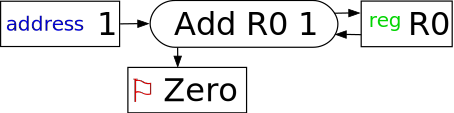
\includegraphics[scale=0.3]{fig/add.pdf}
 \end{minipage}
\end{figure}

\noindent
To implement \hs{getProgramEffects}, we apply the natural transformation
\hs{toOver} to the effects of a \hs{Program}, which recursively collects the
effects that occur in the \hs{Write}'s argument \hs{fv}:

\vspace{1mm}
\begin{minted}[xleftmargin=10pt]{haskell}
getProgramEffects :: Program a -> [RW ()]
getProgramEffects = getOver . runSelect toOver
\end{minted}
\vspace{1mm}
\begin{minted}[xleftmargin=10pt]{haskell}
toOver :: RW a -> Over [RW ()] a
toOver (Read  k _   ) = Over [Read k (const ())]
toOver (Write k fv _) = runSelect toOver fv *> Over [Write k fv (const ())]
\end{minted}
\vspace{1mm}

\noindent
The semantics of the addition instruction has only used applicative combinators
and we thus could have analysed it statically using free applicative functors.
However, there are important instructions whose semantics cannot be expressed
in terms of the \hs{Applicative} interface, and this is where the presented
free selective construction becomes irreplaceable.

\subsubsection{Example 2. Conditional Jump}

Selective functors introduce limited dependencies between effectful
computations, giving us enough power to express the semantics of branching
instructions, which modify the program counter by a given offset if a certain
condition holds. Consider the following instruction that performs a jump if the
result of the previous operation was zero.

\vspace{1mm}
\begin{minted}[xleftmargin=10pt]{haskell}
jumpZero :: Value -> Program ()
jumpZero offset = let zeroSet  = (==1) <$> read (Flag Zero)
                      modifyPC = void $ write PC ((+offset) <$> read PC)
                  in whenS zeroSet modifyPC
\end{minted}
\vspace{1mm}

\noindent
Here we use the \hs{whenS} combinator to modify the program counter only if
the \hs{Zero} flag is set. By implementing \hs{jumpZero} in terms of the
selective interface, we achieve both the ability to implement an adequate
simulator for branching programs and perform their static analysis:

\vspace{1mm}
\begin{figure}[!h]
 \begin{minipage}{0.45\textwidth}
\raggedleft
\begin{minted}[xleftmargin=7pt]{haskell}
@\ghci@ getProgramEffects (jumpZero 42)
[Read Zero,Read PC,Write PC]
\end{minted}
 \end{minipage}
 \begin{minipage}{0.54\textwidth}
  \centering
  
\includegraphics[scale=0.3]{fig/jumpZero.pdf}
 \end{minipage}
\end{figure}
\vspace{1mm}

\noindent
Since the analysis is static, the resulting list of effects and the
corresponding data flow graph are over-approximations and show all effects that
can possibly happen during the execution.

% Note that it does not matter which argument we supply to \hs{jumpZero}, since
% it will never get forced, e.g. the analysis will succeed and give us the same
% result even if we supply \hs{undefined}.

\subsubsection{Example 3. Blocks of Instructions}

Once we have implemented the semantics for a desired subset of an ISA, we can
describe the semantics of sequences, or \emph{blocks}, of instructions by
simply composing the semantics of individual instructions using the applicative
sequencing operator (\hs{*>}):

% \vspace{1mm}
\begin{minted}[xleftmargin=10pt]{haskell}
addAndJump :: Program ()
addAndJump = add R0 1 *> jumpZero 42
\end{minted}
\vspace{1mm}

\noindent
We can analyse such compound computations in the same way as we analyse
individual instructions:

\vspace{-1mm}
\begin{figure}[!h]
 \begin{minipage}{0.46\textwidth}
\raggedleft
\begin{minted}{haskell}
@\ghci@ getProgramEffects addAndJump
[Read R0,Read 1,Write R0,Write Zero
,Read Zero,Read PC,Write PC]
\end{minted}
 \end{minipage}
 \begin{minipage}{0.50\textwidth}
  \centering
  
\includegraphics[scale=0.3]{fig/addAndJump.pdf}
 \end{minipage}
\end{figure}
\vspace{-1mm}

% Getting a flat list of effects that blocks of code perform is not very useful,
% since they does not carry any explicit data-flow information. To mitigate this
% restriction, we take the following approach. We create a (1) deeply-embedded
% assembly language and (2) implement an interpreter which assigns a semantics to
% this language in terms of the free selective construction. By doing this, we can
% then implement a mechanical procedure which would construct \emph{data flow
% graphs} of sequences of instructions, similar to the ones shown in
% Fig.~\ref{fig-addAndJump-gcd} by overlaying the graphs for single instructions.
% Note that if an instruction performs multiple read/writes of the same location,
% we will deliberately merge them in the resulting graph.

\subsubsection{Simulation}

To implement an ISA simulator, we follow the same path as in the \hs{pingPongS}
example and the \hs{IO} monad earlier in~\S\ref{sec-free-ping-pong}. We need a
natural transformation from the base functor \hs{RW} to an appropriate target
functor, e.g. an instance of \hs{MonadState}~\hs{ISAState}, where \hs{ISAState}
represents the state of all registers, memory cells and flags. For brevity, we
present only one part of such a transformation, which assigns an interpretation
to reading and writing of register keys~\hs{Reg}:

\vspace{1mm}
\begin{minted}[xleftmargin=10pt]{haskell}
toState :: MonadState ISAState m => RW a -> m a
toState (Read k t) = t <$> case k of
    Reg r -> (Map.! r) <$> gets registers -- Look up r in the registers field
    ...
toState (Write k fv t) = case k of
    Reg r -> do v <- runSelect toState fv -- Evaluate the Write's argument
                let step s = Map.insert r v (registers s)
                state $ \s -> (t v, s { registers = step s })
    ...
\end{minted}
\vspace{1mm}

\noindent
To read a register, we simply lift the lookup function \hs{Map.!} to the
corresponding field of the \hs{ISAState}. To write an effectful value \hs{fv}
into a register, we need to evaluate it first; hence we call the \hs{runSelect}
function, supplying it the natural transformation \hs{toState}, recursively,
thus performing the effects of \hs{fv}. We then adjust the register bank with
the new value and return it.

The natural transformation \hs{toState} gives interpretation to individual
\hs{Read} and \hs{Write} commands, and now this interpretation can be extended
to any \hs{Program} by plugging it into a \hs{runSelect} call, as has already
been done once in the implementation of \hs{toState} itself:

\vspace{1mm}
\begin{minted}[xleftmargin=10pt]{haskell}
runProgram :: Program a -> ISAState -> (a, ISAState)
runProgram p = runState (runSelect toState p)
\end{minted}

\subsubsection{Limitations}

The free selective construction in combination with the base functor \hs{RW}
provides an abstraction capable of expressing the semantics of arithmetic,
load/store and branching instructions. However, one should remember that
selective functors still lack the full expressive power of the monadic interface
and are unable to accommodate an important class of instructions, specifically
those that use the \emph{memory-indirect addressing mode}. If we had a
\hs{Monad}~\hs{Program} instance, we could give the following semantics to the
memory-indirect load instruction \hs{loadMI}:

\vspace{1mm}
\begin{minted}[xleftmargin=10pt]{haskell}
loadMI :: Register -> Address -> Program Value
loadMI reg addr = read (Cell addr) >>= \x -> write (Reg reg) (read (Cell x))
\end{minted}
\vspace{1mm}

\noindent
Here, we read from a memory cell \hs{addr}, then use the monadic bind operator
to extract a value~\hs{x} from the result, and use it in a subsequent memory
read \emph{as address}. Although this semantics is, in principle, implementable
using the selective \hs{bindS} combinator (see \S\ref{sec-alt-multi}), it is not
very useful in practice since static analysis would record possible access to
\emph{all memory cells}~\hs{x}, and there are too many of them (typically, a
large power of two). Furthermore, the execution of the resulting semantics would
be terribly slow, since it would also follow the same linear exploration of the
memory address space (although see \S\ref{sec-alt-multi} for a possible solution
of the performance issue).

% not get any strong benefits. Specifically, since the \hs{getProgramEffects} function,
% which performs static analysis of effects, constructs a conservative
% over-approximation, it would always report something similar to this:
% \hs{[Read addr,Write reg, Write reg...}, which would contain as much instances
% of the \hs{Write} effects as much inhabitants there are in the address
% datatype (usually a large power of two).  Therefore, we lose static analysis.
% Maybe we could get some benefit in simulation? No, unfortunately we, again,
% will not, since \hs{bindS} cannot get magically translated to the monadic
% \hs{>>=}, but instead performs explicit enumeration of inhabitants of the
% bound variable's type, which causes terrible performance regression comparing
% to a monadic implementation. Considering these arguments, using \hs{bindS} for
% mimicking monadic behaviour is not feasible in our case and memory-indirect
% load cannot be modelled in by means of the \hs{ISA} datatype.

\section{Alternative formulations for selective functors}
\label{sec-alternatives}

This section discusses two alternative formulations for selective functors:
adding multi-way generalisations of \hs{select} to the \hs{Selective} type
class (\S\ref{sec-alt-multi}), and making \hs{select} more
symmetric~(\S\ref{sec-alt-symmetric}). Both of these ideas can be readily
integrated into the presented definition of the \hs{Selective} type class by
extending it with new methods and adding new laws that ensure that the
new methods interact with \hs{select} in an appropriate manner. This is common
in standard Haskell libraries, where type classes \hs{Applicative} and
\hs{Monad} include methods like \hs{*>} and \hs{>>} for performance reasons.

% incorporating \hs{select} to \hs{Applicative} (\S\ref{sec-alt-applicative}),

Another alternative that is worth a brief discussion is to simply add the
\hs{select} method to the \hs{Applicative} type class, with the default
implementation \hs{select}~\hs{=}~\hs{selectA}. While this is a viable approach
from the technical viewpoint, it would make it harder to reason about code with
the \hs{Applicative}~\hs{f} constraint, since the \hs{select} method makes it
possible for effects to depend on values; declaring such a significant ability
by the \hs{Selective}~\hs{f} constraint is arguably a more prudent approach.

\subsection{Multiway select operators}\label{sec-alt-multi}

As discussed in~\S\ref{sec-selective}, \hs{branch} is a strong contender to be
the main method of the \hs{Selective} type class: it is parametric and all
selective combinators, including \hs{select} itself, can be derived from it:

\vspace{1mm}
\begin{minted}[xleftmargin=10pt]{haskell}
branch :: Selective f => f (Either a b) -> f (a -> c) -> f (b -> c) -> f c

selectB :: Selective f => f (Either a b) -> f (a -> b) -> f b
selectB x y = branch x y (pure id)
\end{minted}
\vspace{1mm}

\noindent
While we prefer \hs{select} for its simplicity, \hs{branch} does provide an
interesting advantage in the context of static analysis. Specifically, it makes
it statically apparent that the two branches are \emph{mutually exclusive}. When
\hs{branch} is ``desugared'' into a sequence of two \hs{select} operations, the
information about the mutual exclusion between the two branches is lost, which
rules out some static analysis scenarios. For example, it may be useful to know
that in our build systems example in~\S\ref{sec-static-example} we never depend
on both \cmd{lib.c} and \cmd{lib.ml}.

Another point in favour of \hs{branch} is performance: the \hs{select}-based
implementation of the \hs{ifS} combinator checks for the \hs{Left} and
\hs{Right} cases in sequence, instead of directly jumping to the correct case,
so a \hs{branch}-based implementation would be more efficient. Furthermore,
$N$-way generalisations of \hs{select} are possible, although the design space
here is quite large. As an example, one might consider adding \hs{bindS} to the
\hs{Selective} type class, i.e. a special case of the monadic bind operator that
is applicable only to enumerable types:

\vspace{1mm}
\begin{minted}[xleftmargin=10pt]{haskell}
bindS :: (Bounded a, Enum a, Eq a) => f a -> (a -> f b) -> f b
\end{minted}
\vspace{1mm}

\noindent
The default implementation could be based on sequentially checking for every
possible value using \hs{select}, but monadic instances would supply a much
faster implementation, namely \hs{bindS}~\hs{=}~\hs{(>>=)}. This would allow
static analysis instances to capture all possible dependencies without incurring
$O(N)$ slowdown during the execution of an $N$-way branch.

Interestingly, adding the ability to branch on infinite number of cases makes
selective functors equivalent to monads, although it is worth pointing out that
static analysis of such infinitely-branching selective functors might take
infinite time too.

Investigation of the design space for ``multiway selective functors'', and
exploiting it for efficient translation of Haskell's \cmd{do}-notation into
selective functors in the spirit of the \cmd{ApplicativeDo}
extension~\citep{marlow2016applicativedo} is left for future work. For now, we
believe that adding \hs{branch} and/or an equivalent of \hs{bindS} into the
\hs{Selective} type class would be beneficial for performance-sensitive
applications.

\subsection{Symmetric select operators}\label{sec-alt-symmetric}


% Arseniy's raise/catch

% Loops

\section{Related work}\label{sec-related}

Composing effectful computations is a rich research area and there is a vast
body of related work. We build on the fundamental notions of applicative
functors~\citep{mcbride2008applicative} and
monads~\citep{moggi1991notions,1995_wadler_monads}, but these notions are not
isolated: the space between them is inhabited by
\emph{arrows}~\citep{hughes2000arrows} and \emph{generalised
arrows}~\citep{megacz2011hardware}, which we discuss in~\S\ref{sec-arrows}.

The idea of extending the \hs{Applicative} interface to gain more expressive
power is of course not new, and has been particularly popular in
the area of \emph{applicative parser combinators}. In particular,
\citet{swierstra1996parsers} used an extended version of applicative functors
that was later abstracted into the \hs{Alternative} type class, which is
discussed in~\S\ref{sec-alternative-functors}. Other extensions include
combinators for \emph{observable recursion}, e.g.
see~\citep{devriese2012finally,devriese2013fixing}. Combining the latter with
selective functors would give us the ability to statically analyse effectful
computations with cycles.

Our free construction for rigid selective functors is inspired by the works
on free applicative functors~\citep{free-applicatives} and free
monads~\citep{swierstra2008data}, as well as by insightful blog posts
by~\citet{fancher2016free,fancher2017static}.

\subsection{Arrows and profunctors}\label{sec-arrows}

Arrows, introduced by~\citet{hughes2000arrows}, generalise monads by making the
\emph{input} of a computation explicit. Rather than giving the type
\hs{f}~\hs{a} to an effectful computation that yields a value of type~\hs{a}, as
we have done in this paper so far, arrows give the type \hs{a}~\hs{i}~\hs{o} to
an effectful computation that takes values of type \hs{i} as input and yields
values of type \hs{o} as output. There is a rich \emph{arrow hierarchy} of type
classes, each providing a new ability, where \hs{ArrowChoice} is particularly
relevant for us:

\vspace{1mm}
\begin{minted}[xleftmargin=10pt,fontsize=\small]{haskell}
class Category a                  -- identity arrow, sequential arrow composition
class Category a => Arrow       a -- pure arrows, parallel arrow composition
class Arrow    a => ArrowChoice a -- arrows with choice
class Arrow    a => ArrowApply  a -- arrows that take arrows as input
class Arrow    a => ArrowLoop   a -- arrows with loops
\end{minted}
\vspace{1mm}

\noindent
The relationships between applicative functors, monads and arrows have been
studied in depth. It is known, e.g. see~\citet{lindley2011idioms}
and~\citet{rivas2017notions}, that applicative functors correspond to so called
\emph{static arrows}, for which there is an isomorphism between
\hs{a}~\hs{()}~\hs{(}\hs{i}~\hs{->}~\hs{o)} and~\hs{a}~\hs{i}~\hs{o}. The
standard module \textsf{Control.Arrow} therefore provides the following
definitions:

\vspace{1mm}
\begin{minted}[xleftmargin=10pt]{haskell}
newtype ArrowMonad a b = ArrowMonad (a () b) -- See Control.Arrow

instance Arrow      a => Functor     (ArrowMonad a)
instance Arrow      a => Applicative (ArrowMonad a)
instance ArrowApply a => Monad       (ArrowMonad a)
\end{minted}
\vspace{1mm}

\noindent
Selective functors provide the missing equivalent for \hs{ArrowChoice} in the
\emph{functor hierarchy}, as demonstrated by the following instance:

\vspace{1mm}
\begin{minted}[xleftmargin=10pt]{haskell}
instance ArrowChoice a => Selective (ArrowMonad a) where
    select (ArrowMonad x) y = ArrowMonad $ x >>> (toArrow y ||| returnA)

toArrow :: Arrow a => ArrowMonad a (b -> c) -> a b c
toArrow (ArrowMonad f) = arr (\x -> ((), x)) >>> first f >>> arr (uncurry ($))
\end{minted}
\vspace{1mm}

\noindent
Here \hs{toArrow} witnesses one half of the aforementioned isomorphism between
\hs{a}~\hs{()}~\hs{(}\hs{i}~\hs{->}~\hs{o)} and~\hs{a}~\hs{i}~\hs{o}. The
obtained \hs{Selective} instance is lawful thanks to the \hs{ArrowChoice} laws.

\emph{Profunctors} is an abstraction closely related to arrows;
see~\citep{pickering2017profunctor} for a good overview of profunctors in the
context of modular data accessors, or \emph{lenses}. Similarly to
\hs{ArrowChoice}, so-called \emph{Cocartesian profunctors} are counterparts of
selective functors in the \emph{profunctor hierarchy}.

Establishing a formal correspondence between \hs{ArrowChoice}, Cocartesian
profunctors, and selective functors is beyond the scope of this paper and is
left for future research.

\subsection{Parsers and \hs{Alternative} type class}\label{sec-alternative-functors}

\hs{Alternative} is a type class originally motivated by non-monadic parsers;
see, for example,~\citet{swierstra1996parsers}, where the methods of the
\hs{Alternative} type class appear as part a bigger \hs{Parsing} type class. In
modern Haskell, \hs{Alternative} is a subclass of \hs{Applicative}:

\vspace{1mm}
\begin{minted}[xleftmargin=10pt]{haskell}
class Applicative f => Alternative f where
    empty :: f a
    (<|>) :: f a -> f a -> f a
\end{minted}
\vspace{1mm}

\noindent
The operator \hs{<|>} allows us to naturally express \emph{choice} in parsers.
As an example, consider the task of parsing binary and hexadecimal numbers,
which are prefixed with \hs{"0b"} and \hs{"0x"}, respectively. Following the
classic parser combinator approach~\citep{hutton1998monadic}, let us assume the
existence of the following parsers:

\vspace{1mm}
\begin{minted}[xleftmargin=10pt]{haskell}
sat    :: (Char -> Bool) -> Parser Char   -- parse a specified character
string :: String         -> Parser String -- parse a string literal
bin    ::                   Parser Int    -- parse a binary-encoded number
hex    ::                   Parser Int    -- parse a hexadecimal-encoded number
\end{minted}
\vspace{1mm}

\noindent
Now the desired parser can be obtained as a choice between parsers for binary
and hexadecimal numbers, each augmented with the prefix-parsing part:

\vspace{1mm}
\begin{minted}[xleftmargin=10pt]{haskell}
numberA :: Parser Int
numberA = (string "0b" *> bin) <|> (string "0x" *> hex)
\end{minted}
\vspace{1mm}

\noindent
When parsing \hs{"0x7E3"}, the first parser fails (due to the prefix mismatch),
but the second one succeeds. Note that parsing of the leading \hs{"0"} can be
factored out into a separate parser \hs{string}~\hs{"0"} to avoid backtracking.

Selective functors also allow us to implement the desired parser, and arguably
in a more direct style that does not involve trying one parser after another:

\vspace{1mm}
\begin{minted}[xleftmargin=10pt]{haskell}
numberS :: Parser Int
numberS = ifS ((== 'b') <$> (string "0" *> sat (`elem` "bh"))) bin hex
\end{minted}
\vspace{1mm}

\noindent
Here we first parse the leading \hs{"0"}, then the second character of the
prefix, failing if it is neither \hs{"b"} nor \hs{"h"}, and finally select an
appropriate subsequent parser using \hs{ifS}.

Investigation of the relationship between \hs{Alternative} and \hs{Selective}
type classes, as well as application of selective functors to parsers is left
for future work.

% Anything else?
% Kleisli functors
% https://elvishjerricco.github.io/2016/10/12/kleisli-functors.html

\section{Conclusions}\label{sec-conclusions}

We have introduced selective functors, an abstraction between applicative
functors and monads. Like applicative functors, selective functors require all
effects to be known statically, before the execution starts. Like monads,
selective functors allow for effects to depend on values of earlier effects but
in a limited way: it is possible to skip some of the effects, but not create
new ones. In this sense selective functors allow you to describe computations
that are very much like hardware circuits: statically fixed, yet dynamically
reconfigurable.

We have demonstrated usefulness of the new abstraction on several examples, and
hope that the reader will find it useful in their next project too.


\begin{acks}
  %% Commands \grantsponsor{<sponsorID>}{<name>}{<url>} and
  %% \grantnum[<url>]{<sponsorID>}{<number>} should be used to
  %% acknowledge financial support and will be used by metadata
  %% extraction tools.
  We are very grateful to everyone who contributed by participating in numerous
  discussions and providing feedback on earlier drafts of this paper.

  Arseniy Alekseyev, Ulan Degenbaev and Neil Mitchell have been closely
  following the work on selective functors from the very first blog post; their
  early and constructive feedback encouraged and guided our research.

  Many others have joined and helped as the work progressed, including:
  Thorsten Altenkirch, \mbox{Baldur} Bl{\"o}ndal, Dominique Devriese,
  Ivan Gotovchits, Oleg Grenrus, Jennifer Hackett, Graham Hutton,
  Luka Jacobowitz, Edward Kmett, Lennox S. Leary, G\'abor Lehel, Sam Lindley,
  Tim McGilchrist, James McKinna, Yaron Minsky, Alexandre Moine, Matthew Naylor,
  Daniel Peebles, Artem Pelenitsyn, Simon Peyton Jones, Ivan Polyakov,
  Gabriel Radanne, Asad Saeeduddin, Irakli Safareli, Carter Schonwald,
  Danil Sokolov, Ian Treyball, Anton Trunov, Cristian Urlea, Sjoerd Visscher,
  Alexa de Wit, Brent Yorgey, Vladislav Zavialov, and reddit users
  \cmd{Darwin226}, \cmd{dmwit}, \cmd{sclv}, \cmd{viercc} and \cmd{yakrar}. With
  such an active and helpful community, we are certain that the above list is
  just an under-approximation of all our interactions, and we apologise for any
  omissions.

  Last but not least, we would like to thank the four ICFP reviewers who
  discovered and helped to fix a few important issues in the submitted version
  of the paper.

  Andrey Mokhov's research is supported by a Royal Society Industry Fellowship
  \cmd{IF160117} on the topic ``Towards Cloud Build Systems with Dynamic
  Dependency Graphs''.
\end{acks}

\newpage
\bibliography{refs}
\end{document}
